\documentclass[utf8, diplomski, lmodern, numeric]{fer}

\usepackage{booktabs}

\usepackage{float}

\usepackage{chngpage}

\usepackage[export]{adjustbox}

\usepackage{listings}
\renewcommand{\lstlistingname}{Programski isječak}
\renewcommand{\lstlistlistingname}{Lista programskih isječaka}

\usepackage[dvipsnames]{xcolor}
\definecolor{backcolour}{rgb}{0.90,0.90,0.90}

\usepackage{indentfirst}
\setlength{\parindent}{10mm}
\setlength{\parskip}{2mm}



\begin{document}

\thesisnumber{1954}

\title{Stvarnovremensko praćenje parametara ispravnosti rada u sustavu za raspodijeljenu obradu tokova podataka}

\author{Mislav Jakšić}

\maketitle

\begin{figure}[H]
    \centering
    \hspace*{-35mm}
    
\includegraphics{task.pdf}
\end{figure}

\zahvala{}

\tableofcontents



\chapter{Uvod}

Raspodijeljeni sustavi su nepouzdani. Pogreška u sklopovlju, operacijskom sustavu, programu ili mreži može izazvati ispad bilo kojeg dijela sustava. Ispadi u raspodijeljenom sustavu mogu pokrenuti lanac ispada. Ako ispad ne uzrokuje lanac ispada sustav će i dalje patiti jer će program i dalje zahtijevati računalno vrijeme i memoriju, a s njima neće obavljati koristan posao. U najgorem slučaju ispad može izazvati potpuno zatajenje sustava gdje je jedini lijek iznova pokrenuti sve njegove dijelove. U najboljem slučaju ispad će samo smanjiti učinkovitost sustava. Bez pažljivog nadzora raspodijeljenog sustava ispad je teško otkriti te još teže otkloniti izvor ispada.

Zadatak nadzora je otkriti ispad i njegov uzrok. Ispadi se dijele na ispad procesa, pogreške u komunikaciji, vremenske pogreške, pogrešan odgovor i bizantske pogreške \citep{rassus-manual}. Ako se ispad želi otkriti potrebno je pratiti vrijednosti koje ukazuju da se ispad dogodio. Korisne vrijednosti mogu biti zauzeće memorije, brzina obrade zahtjeva, sadržaj poruke ili duljina uspostave komunikacijskog kanala. Nadzirani program vrijednosti predaje nadzorniku koji je čovjek ili program. Ako nadzor obavlja program on treba biti pouzdaniji od nadziranog programa inače je problem nadzora udvostručen, a ne riješen.

Prvi korak u izradi pouzdanog sustava nadzora je izrada pouzdanog sakupljača vrijednosti. Prije izrade sakupljača u poglavlju 2 uspoređeni su predstavnici sustava za raspodijeljenu obradu podataka. Nakon usporedbe u poglavlju 3 opisane su pretpostavke i zahtjevi, dok poglavlje 4 uspoređuje postojeće sakupljače vrijednosti sa specifikacijom problema. U poglavlju 5 opisana je arhitektura, a u poglavlju 6 programska izvedba sakupljača vrijednosti za programski alat Apache Kafka koji potiskuje pročitane vrijednosti prema udaljenom nadzornom sustavu.



\chapter{Sustavi za raspodijeljenu obradu tokova podataka}

Tok podataka \engl{data stream} nije isto što i skup podataka \citep{ilprints535}. Toku podataka podaci dolaze stalno, u nepoznatom redoslijedu, bez znaka kada će prestati i bit će odbačeni nakon što su pročitani. Ovi sustavi su raspodijeljeni jer se tok mora obraditi brzo. Primjer problema toka podataka su kartično plaćanje, praćenje korisnika mrežnih stranica, posluživanje reklama i preporuka. Svi navedeni problemi imaju mnogo izvora i ponora podataka. Kako sakupiti, zabilježiti, te dostaviti podatke u ponor gdje će se obraditi su problemi za koje sustavi za raspodijeljenu obradu tokova podataka nude rješenje. Zato što su tokovi podatka raznovrsni razvijeno je mnogo alata za njihovu obradu. Alate razlikujemo po načinu sakupljanja podataka, po mogućnostima obrade toka podataka, po arhitekturi i načinu zapisivanja podataka.

Prije izvedbe sakupljača vrijednosti potrebno je usporediti i izabrati alat za raspodijeljenu obradu podataka. Kako bi usporedba alata i izvedba sakupljača bila jednostavnija u obzir su uzeti samo javno dostupni alati. Većina takvih alata koristi model objavi/pretplati. Umjesto da se usporede svi javno dostupni alati izabran je predstavnik iz svakog važnog skupa alata:
\begin{itemize}
    \item Apache Kafka je predstavnik popularnih alata za raspodijeljenu obradu tokova podataka
    \item Apache Pulsar \citep{yahoo-blogpost} je predstavnik modernih alata objavljen 2016. dok je Kafka \citep{kafka-whitepaper} objavljena 2011. godine
\end{itemize}


\section{Model objavi/pretplati}

Apache Kafka i Apache Pulsar koriste model objavi/pretplati \engl{publish/subscribe} za razmjenu podataka između procesa. Slika \ref{fig:publish-subscribe} prikazuje dijelove modela objavi/pretplati. Model objavi/pretplati sastoji od objavljivača \engl{publisher} koji šalju poruke, pretplatnika \engl{subscriber} koji čitaju poruke i posrednika \engl{broker} koji razmjenjuje poruke između njih \citep{rassus-manual}. Posrednik zapisuje objavljene poruke i dopušta pretplatnicima čitanje poruka. Prednost modela objavi/pretplati nad izravnim razgovorom među procesima je što objavljivači i pretplatnici ne trebaju znati jedan za drugoga.

\begin{figure}[H]
    \centering
    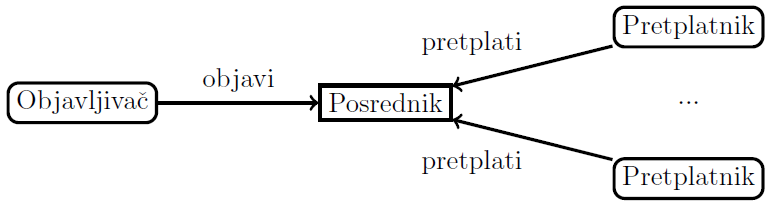
\includegraphics[max width=0.8\textwidth, max height=0.6\textwidth]{PublishSubscribe.png}
    \caption{Model objavi/pretplati}
    \label{fig:publish-subscribe}
\end{figure}


\section{Apache Kafka}

\begin{figure}[H]
    \centering
    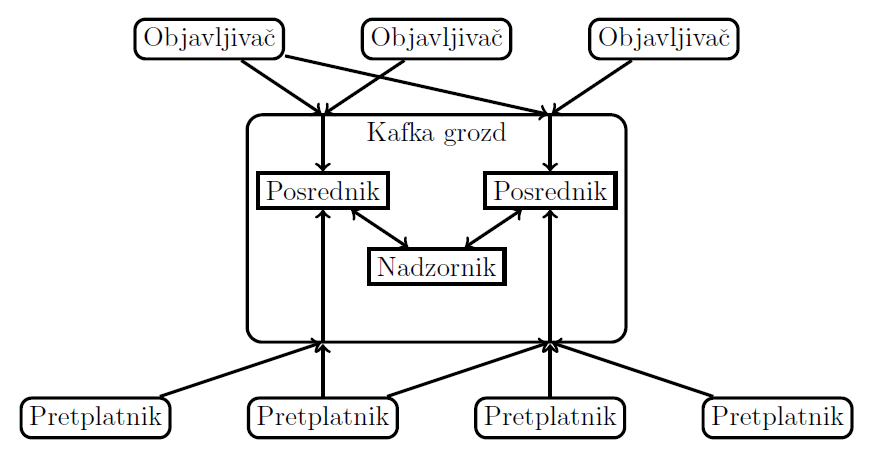
\includegraphics[max width=0.8\textwidth, max height=0.6\textwidth]{KafkaCluster.png}
    \caption{Apache Kafka grozd}
    \label{fig:kafka-cluster}
\end{figure}

Apache Kafka je popularni alat za raspodijeljenu obradu tokova podataka. Slika \ref{fig:kafka-cluster} prikazuje Kafka grozd. Svaki grozd sastoji se od ZooKeeper nadzornika i barem jednog posrednika. Nadzornik usklađuje posrednike. Objavljivači šalju poruke u temu grozda. Posrednici zapisuju poruke u pretinac teme. Pretplatnici čitaju poruke iz teme grozda i obrađuju podatke. Primjena, arhitektura i izvedba Kafka pretplatnika, pretinca, posrednika, teme i objavljivača opisana je u sljedećim poglavljima \citep{kafka-whitepaper} \citep{kafka-docs}.

\subsection{Objavljivač}
Objavljivač \engl{producer} je korisnički program koji šalje poruke u temu grozda. Poruka se obvezno sastoji od sadržaja, teme na koju se objavljuje, oznake pretinca, odmaka u pretincu i vremena objave. Poruke se šalju u skupini nakon što prođe određeno vrijeme ili se nakupi dovoljno poruka. Poruke se mogu sažeti prije slanja \citep{kafka-compression}. Tema je podijeljena na pretince. Pretinac je dnevnik u koji posrednik zapisuje poruke. Posrednik je poslužitelj koji zapisuje poruke u pretinac. Objavljivač ključem izabere pretinac u koji želi zapisati poruke ili poruke šalje u svaki pretinac jednoliko. Posrednik će poslati potvrdu kada se poruke zapišu u pretinac vođe i izabrani broj usklađenih sljedbenika. Prije slanja sljedećeg skupa poruka objavljivač može pričekati potvrdu posrednika.

Ako se dogodi ispad objavljivača ili posrednika, objavljivač će ponovno poslati poruke. Objavljene poruke bit će dostavljene posredniku barem jednom. Ako je uvišestručavanje poruka nedopustivo, objavljivač mora koristiti transakcijski način rada.

\subsection{Tema}
Tema \engl{topic} je tok poruka, apstraktna umotvorina u koju objavljivači šalju poruke, a iz koje pretplatnici čitaju poruke. Posrednici se brinu da poruke budu zapisane. Biti pretplaćen na temu znači napraviti podtok poruka. Poruke objavljene u temi se ravnomjerno raspoređuju u podtokove. Svaki podtok ima pokazivač kojim pretplatnik čita poruke. Ako pokazivač dođe do kraja podtoka, pretplatnik se blokira dok se ne objavi nova poruka. Količina nepročitanih poruka u temi ne utječe na protok poruka kroz temu. Poruke u temi se brišu tek nakon određenog vremena. Tema je podijeljena na pretince iz kojih posrednici čitaju i u koje zapisuju poruke. Kako bi poruke u pretincu bile dostupne nakon ispad posrednika, pretinac je moguće umnožiti.

\subsection{Posrednik}
Posrednik \engl{broker} je poslužiteljski program koji zapisuje poruke objavljivača i poslužuje poruke pretplatnicima. Svaki posrednik dio je samo jednog Kafka grozda. Posrednici koriste Apache ZooKeeper za izvršavanje sporazumnog algoritma, pamćenje tema, njihovih pretinaca i usklađenih posrednika. Posrednik će poruke zapisati u pretinac onim redoslijedom kojim je objavljivač poslao poruke, ne redoslijedom kojim je posrednik primio poruke. Pretplatnici će s posrednika čitati poruke onim redoslijedom kojim su zapisane u pretinac.

Kada objavljivač objavi poruke na temu posrednik će zapisati poruke u određeni pretinac. Posrednik koristi sustav straničenja \engl{memory paging} i tvrdi disk za zapisivanje poruka \citep{kafka-paging}. Umjesto da posrednik koristi memoriju procesa za priručnu memoriju posrednik poruke predaje sustavu straničenja operacijskog sustava. Operacijski sustav će poruke zapisati u stranice i pohraniti u nedodijeljene dijelove radne memorije. Poruke se zapisuju na tvrdi disk samo kada operacijski sustav želi osloboditi memoriju sustava straničenja. Opisano gospodarenje memorijom dopušta posredniku da čuva veliku količinu poruka bez gubitka učinkovitosti.

Pretplatnici često dohvaćaju uzastopne poruke pa se one čitaju iz priručne memorije umjesto s tvrdog diska. Zahvaljujući sustavu straničenja priručna memorija sa zapisanim porukama će postojati neko vrijeme nakon ispada posrednika. Korištenjem sustava straničenja za zapisivanje poruka izbjegava se korištenje sakupljača smeća Java virtualnog stroja. Umjesto da se poruke zapišu dva puta, jednom u dodijeljenu memoriju procesa i jednom u sustav straničenja poruke se zapisu samo jednom u sustav straničenja.

Kada pretplatnik želi pročitati poruke posrednik će pronaći, pročitati i poslati poruke pretplatniku. Posrednik s sendfile i zero-copy funkcijama čita poruke iz radne memorije i šalje u memoriju mrežne kartice u jednom koraku \citep{linux-sendfile} \citep{java-zero-copy}. Kako bi se dodatno ubrzao rad posrednici, objavljivači i pretplatnici skupine poruka čitaju, zapisuju i šalju u istom binarnom obliku. Prije slanja poruka pretplatnicima posrednik može sažeti poruke.

\subsection{Pretinac}

Pretinac \engl{partition} je logički dnevnik \engl{log} i najmanja gradivna jedinica teme. Kada objavljivač objavi poruku u temu grozda posrednik poruke zapiše u pretinac teme. Slika \ref{fig:kafka-log} prikazuje dnevnik izveden kao skup datoteka iste veličine. Kada posrednik zapiše poruke u pretinac on doda poruke na kraj datoteke. Datoteke se predaju sustavu straničenja operacijskog sustava tek nakon određenog vremena ili broja dodavanja. Svaka poruka ima jedinstvenu oznaku koja je ujedno i odmak unutar datoteke. Odmak sljedeće poruke računa se kao zbroj odmaka i veličine ranije poruke. Zato su oznake poruka jedinstvene i strogo rastuće ali nisu uzastopne.

\begin{figure}[H]
    \centering
    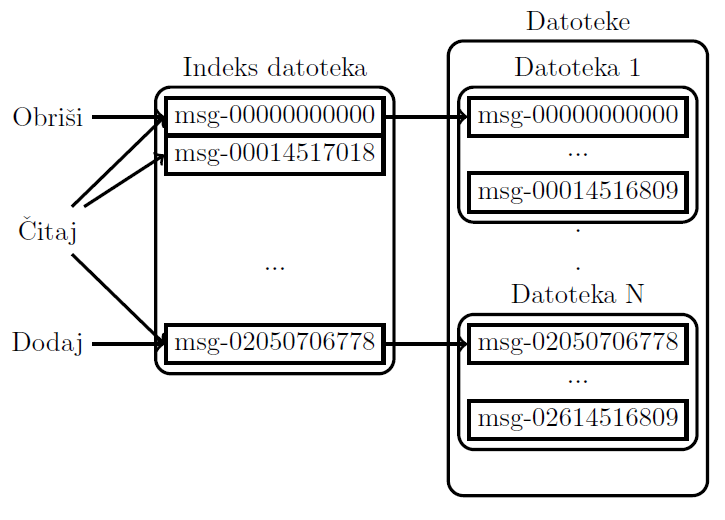
\includegraphics[max width=0.8\textwidth, max height=0.6\textwidth]{KafkaLog.png}
    \caption{Kafka dnevnik}
    \label{fig:kafka-log}
\end{figure}

Protok poruka kroz temu može biti toliki da izazove preopterećenje posrednika. Zato je temu moguće podijeliti na više pretinaca. Ako je B broj posrednika u Kafka grozdu onda tema može biti podijeljena na najviše B pretinaca. Svaki pretinac teme mora biti dodijeljen različitom posredniku.

Ako se dogodi ispad posrednika, poruke u pretincu postat će nedostupne. Ako poruke moraju biti dostupne čak i tijekom ispada posrednika pretinac se mora umnožiti \engl{replicate}. Svaki pretinac može biti umnožen najviše B puta ako je B broj posrednika u Kafka grozdu. Svaki umnoženi pretinac \engl{replica} bit će dodijeljen različitom posredniku jer dodjela istom ne povećava dostupnost uslijed ispada. Ako se pretinac umnoži B puta onda će poruke u pretincu postati nedostupne tek ako se dogodi strogo više od B-1 ispada posrednika.

Kada su pretinci umnoženi potrebno je ujednačiti poruke u svakom umnoženom pretincu. Zato će jedan posrednik biti vođa pretinca \engl{partition leader}, a ostali posrednici će biti pratitelji pretinca \engl{partition follower}. Svaki posrednik može biti vođa najviše jednog pretinca po temi. Vođa pretinca je jedini posrednik koji smije čitati ili pisati poruke u pretinac. Zadaća pratitelja je preusmjeriti korisnike na vođu pretinca i uskladiti svoj pretinac s pretincem vođe. Pratitelji mogu preusmjeriti korisnike na vođu pretinca tako da pitaju ZooKeepera tko je vođa kojeg pretinca. Svaki pratitelj ima pretplatnika koji čita poruke iz pretinca vođe i zapisuje poruke u umnoženi pretinac.

\begin{figure}[H]
    \centering
    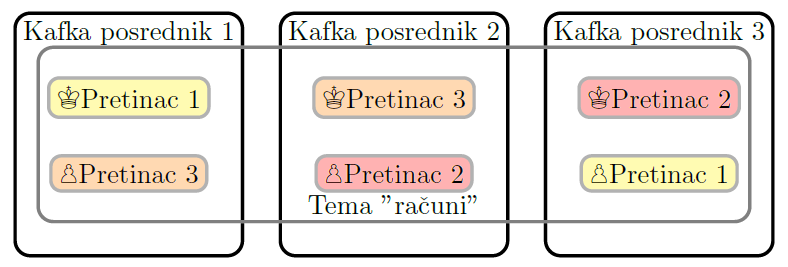
\includegraphics[max width=0.8\textwidth, max height=0.6\textwidth]{KafkaPartitions.png}
    \caption{Pretinci vođe i pretinci sljedbenici}
    \label{fig:kafka-leader-follower}
\end{figure}

Slika \ref{fig:kafka-leader-follower} prikazuje tri posrednika u grozdu. Tema "računi" je podijeljena na najveći mogući broj pretinaca, broj posrednika u grozdu. Kako se poruke ne bi izgubile zbog ispada posrednika svaki pretinac teme je umnožen jednom. Vođa žutog pretinca je nasumično posrednik jedan. Vođa crvenog pretinca će biti ili posrednik dva ili tri jer se vodstvo pretinaca mora jednoliko raspodijeliti. Ako vođa crvenog pretinca postane posrednik tri, onda će vođa narančastog pretinca postati posrednik dva. Pretinci pratitelji rasporede se ravnomjerno po posrednicima tako da pratitelji nikad nisu s vođom u istom posredniku.

Osim što je vođa pretinca jedini posrednik koji može čitati ili pisati poruke u pretinac, on mora brinuti o pratiteljima. Vođa smatra da pratitelj postoji samo ako je prijavljen u Kafka grozd i ako ne zaostaje s čitanjem poruka iz pretinca vođe. Ako zaostaje, vođa će pratitelja izbaciti iz skupa usklađenih pratitelja \engl{in-sync replica}. Kada vođa primi poruke od objavljivača on će poruke zapisati u svoj pretinac i čekat će potvrde pratitelja. Nakon što svi pratitelji pročitaju i zapišu poruke u svoj pretinac vođa pretinca će poslati potvrdu objavljivaču. Pretplatnici mogu čitati samo one poruke koje su i vođa i pratitelji zapisali u svoje pretince.

Ako se posredniku koji je vođa pretinca dogodi ispad, nitko neće moći čitati ili pisati poruke u pretinac. Zato će pratitelji glasati tko će od pratitelja postati novi vođa pretinca. Samo pratitelji koji su u skupu usklađenih pratitelja mogu postati novi vođa. U iznimnom slučaju kada ne postoji usklađeni pratitelj neusklađeni pratitelj može postati novi vođa pretinca.

Posrednika, tema, pretinaca i umnoženih pretinaca je puno. Kako posrednici ne bi glasali za novog vođu pretinca za svaki pretinac zasebno jedan od posrednika je zadužen da bude nadglednik glasanja \engl{election controller}. Ako se dogodi ispad posrednika, nadglednik glasanja će ubrzati glasanje novog vođe pretinca.

\subsection{Pretplatnik}

Pretplatnik \engl{consumer} je korisnički program koji čita poruke iz teme. Slika \ref{fig:kafka-consumer-group} prikazuje odnos pretplatnika i teme. Svaki pretplatnik je član samo jedne skupine pretplatnika \engl{consumer group}. Skupina pretplatnika sastojati se od barem jednog člana. Skupina pretplatnika zajedno čita poruke iz teme. Neki pretplatnici u skupu pretplatnika bit će zaduženi za čitanje poruka iz teme. Svaki zaduženi pretplatnik ima barem jedan pretinac iz kojeg jedino on može čitati poruke. Skupina pretplatnika može istovremeno napraviti najviše P čitanja ako je P broj pretinaca i u skupini pretplatnika je barem P članova. Poruke se mogu pročitati jedino iz pretinca vođe. Ako pretplatnik uputi zahtjev za čitanje pratitelju pretinca on će pretplatnika preusmjeriti na vođu pretinca.

\begin{figure}[H]
    \centering
    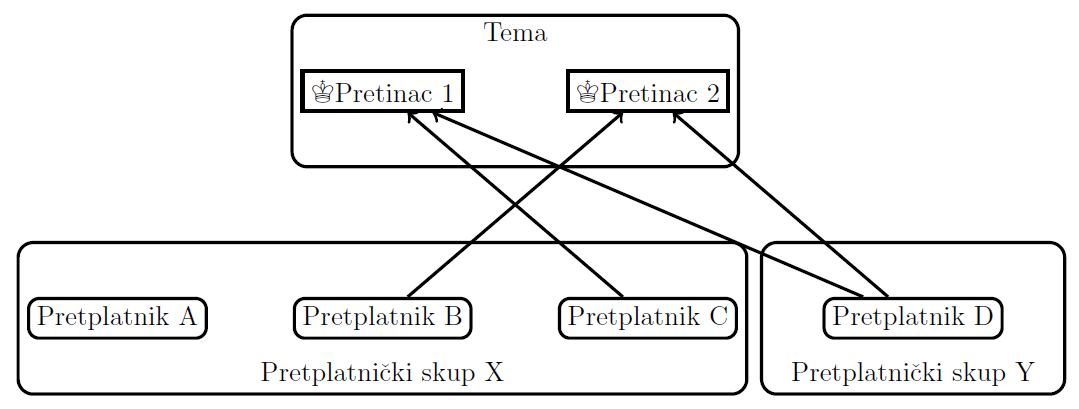
\includegraphics[max width=0.8\textwidth, max height=0.6\textwidth]{KafkaConsumerGroups.png}
    \caption{Kafka pretinci i skup pretplatnika}
    \label{fig:kafka-consumer-group}
\end{figure}

Pretplatnik u zahtjevu za čitanje navodi odmak zadnje pročitane poruke i koliko poruka želi pročitati. Posrednik će dostaviti sve poruke od odmaka do tražene količine ili dok ne dođe do kraja pretinca. Odmak poruke je i jedinstvena oznaka poruke i mjesto u datoteci posrednika gdje se poruka nalazi. Posrednik ne pazi koje je poruke pretplatnik pročitao. Pretplatnik je zadužen za rukovanje odmakom. Odmak zadnje pročitane poruke pretplatnik šalje u posebnu temu posrednika. Ako se dogodi ispad pretplatnika, drugi pretplatnik će pročitati odmak iz teme i nastaviti s čitanjem poruka iz pretinca.

Posrednik će jednom pretplatniku po skupini pretplatnika dostaviti poruku barem jednom. Ako se dogodi ispad pretplatnika ista poruka se može dostaviti više puta. Ako je nedopustivo istu poruku pročitati više puta onda korisnik mora napraviti vlastiti algoritam ili koristiti transakcijskog pretplatnika. Pretplatnik čita poruke onim redoslijedom kojim su poruke zapisne u pretinac. Posrednici vremenski ne uređuju dostavu poruka iz svih pretinaca, ali su poruke vremenski uređene u svakom pretincu pojedinačno. Ako je potrebno vremenski urediti sve poruke u svim pretincima onda je potrebno razviti vlastiti algoritam ili napraviti temu sa samo jednim pretincem.

Više skupina pretplatnika može istovremeno čitati poruke iz iste teme i pretinaca. Posrednik će odaslati \engl{multicast} istu poruku svim pretplaćenim pretplatnicima. Posrednici će skupu pretplatnika omogućiti čitanje poruka samo ako su svi pratitelji u skupu usklađenih pratitelja i vođa pretinca zapisali poruke u pretinac. Nakon što pretplatnik primi poruke on će u temi odmaka ažurirati odmak do kojeg je pročitao poruke.

Model povlačenja \engl{pull model} poruka pretplatnicima dopušta čitanje poruka brzinom koja njima odgovara. Model dopušta i učinkovito slanje iste poruke na više pretplatnika. Ako pretplatnik želi ponovno pročitati poruku on samo treba poslati odmak pročitane poruke. Kako pretplatnik ne bi zapeo u petlji ako u pretincu nema novim poruka on sebe može blokirati dok ne dođu nove poruke. Posrednik nikad ne zna kada su svi pretplatnici pročitali poruke i zato ih ne može obrisati nakon čitanja. Posrednici su zato napravljeni da s povećanjem nepročitanih poruka njihova učinkovitost ne opada. Posrednik će poruke izbrisati nakon zadanog vremena.


\section{Apache Pulsar}

Apache Pulsar je moderni alat za raspodijeljenu obradu tokova podataka. Slika \ref{fig:pulsar-cluster} prikazuje Pulsar proces koji se sastoji od barem jednog Pulsar grozda. Pulsar grozd sastoji se od barem jednog Pulsar posrednika, od barem jednog Apache BookKeeper zapisničara i Apache ZooKeeper nadzornika. Objavljivači šalju poruke u temu grozda. Posrednici primaju i poslužuju poruke, a zapisničari ih zapisuju. Pretplatnici čitaju poruke iz teme grozda i obrađuju podatke. Primjena, arhitektura i izvedba Pulsar pretplatnika, upravljane knjige, posrednika, teme, pretplate i objavljivača opisana je u sljedećim poglavljima \citep{pulsar-docs} \citep{pulsar-streamlio-1} \citep{pulsar-streamlio-2} \citep{pulsar-streamlio-intro}.

\begin{figure}[H]
    \centering
    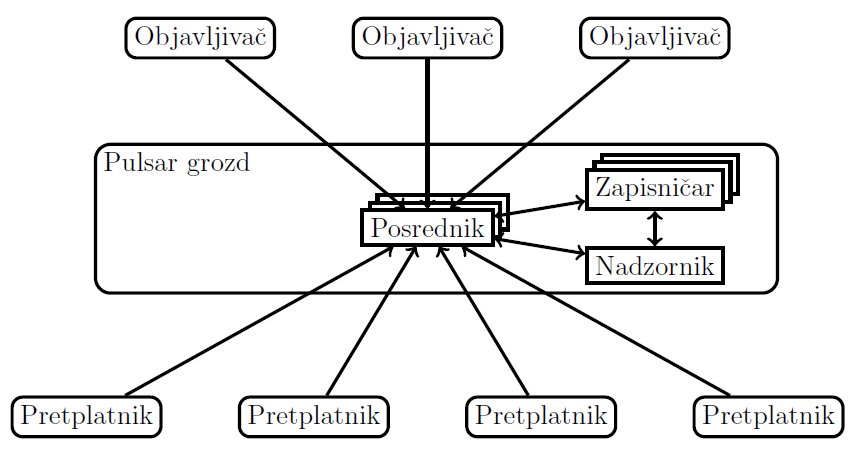
\includegraphics[max width=0.8\textwidth, max height=0.6\textwidth]{PulsarCluster.png}
    \caption{Apache Pulsar grozd}
    \label{fig:pulsar-cluster}
\end{figure}

\subsection{Objavljivač}

Objavljivač je korisnički program koji šalje poruke u temu. Poruke se obvezno sastoje od sadržaja, oznake objavljivača, jedinstvene oznake poruke i vremena objave. Poruke se mogu slati u skupini. Prije slanja, poruke se mogu sažeti. Tema može biti podijeljena na pretince. Objavljivač može usmjeriti poruke u određeni pretinac. Poruke se mogu usmjeriti na jedan nasumični pretinac, na točno određene pretince koristeći ključ ili se mogu slati jednoliko na sve pretince. Objavljivači ili čekaju potvrdu dok posrednik zapisuje poruke ili nastave s radom i naknadno provjere jesu li poruke primljene i zapisane.

\subsection{Tema i pretplata}

\begin{figure}[H]
    \centering
    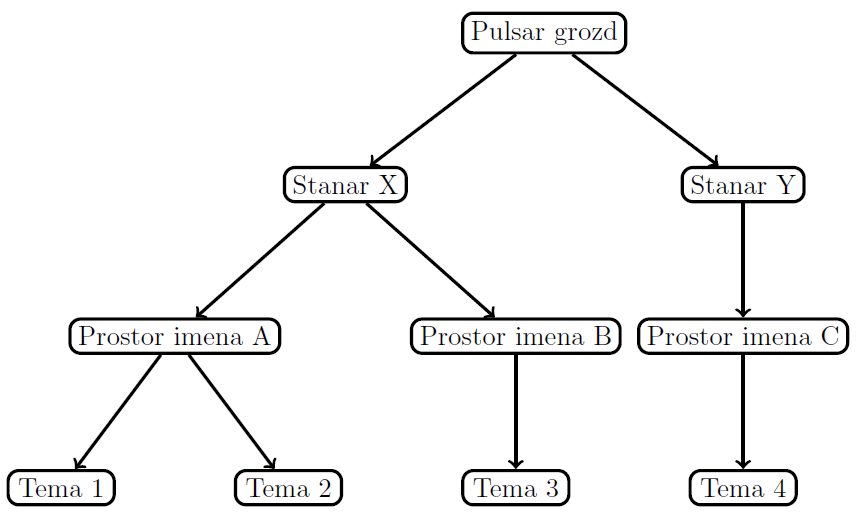
\includegraphics[max width=0.8\textwidth, max height=0.6\textwidth]{PulsarHierarchy.png}
    \caption{Pulsar teme, prostori imena i stanari}
    \label{fig:pulsar-hierarchy}
\end{figure}

Tema je imenovani tok poruka koji prenosi poruke od objavljivača do pretplatnika kroz posrednika. Tema je izgrađena kao poveznica \engl{link}. Slika \ref{fig:pulsar-hierarchy} prikazuje stupnjevanje tema, prostor imena \engl{namespace} i stanara \engl{tenant}. Svaka tema pripada jednom prostoru imena. Prostor imena je upravna jedinka kojom se mijenjaju postavke tema. Svaki prostor imena pripada jednom stanaru. Stanar određuje način pristupa, korištenje resursa, brisanje poruka i izolaciju prostora imena. Stanari pripadaju Pulsar grozdu.

\begin{figure}[H]
    \centering
    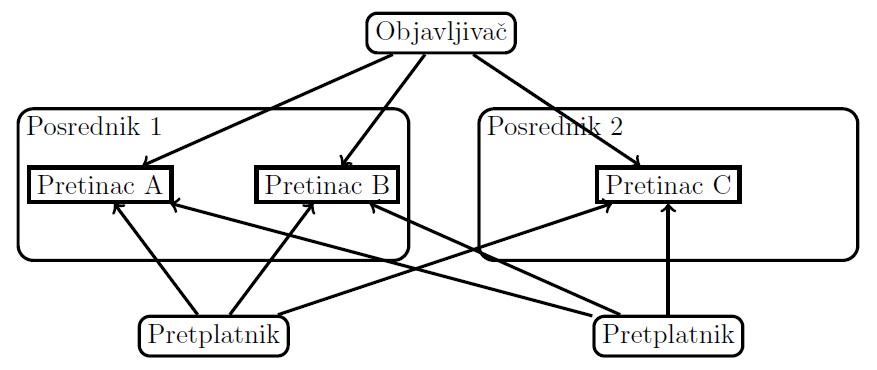
\includegraphics[max width=0.8\textwidth, max height=0.6\textwidth]{PulsarPartitions.png}
    \caption{Pulsar pretinci}
    \label{fig:pulsar-partitions}
\end{figure}

Moguće je napraviti nepostojane teme \engl{non-persistent topics} koje poruke čuvaju do slanja pretplatnicima ili ispada posrednika. Nepostojane teme objavljene poruke potiskuju prema pretplatnicima. Prednost nepostojanih tema je brzina. Količina nepročitanih poruka u temi ne utječe na protok poruka kroz temu. Poruka se briše iz teme kada svi pretplatnici pročitaju poruku ili kada je poruka pročitana i starija od zadane vrijednosti ili kada je nepročitana i starija od zadane vrijednosti. Tema se može podijeliti na više podtema zvanih pretinac. Slika \ref{fig:pulsar-partitions} prikazuje odnos objavljivača i pretplatnika prema temi koja je podijeljena na pretince. Pretinci su ravnomjerno raspodijeljeni po posrednicima. Broj istovremenih pretplatnika odnosno čitanja nije ograničeno brojem pretinaca.

\begin{figure}[H]
    \centering
    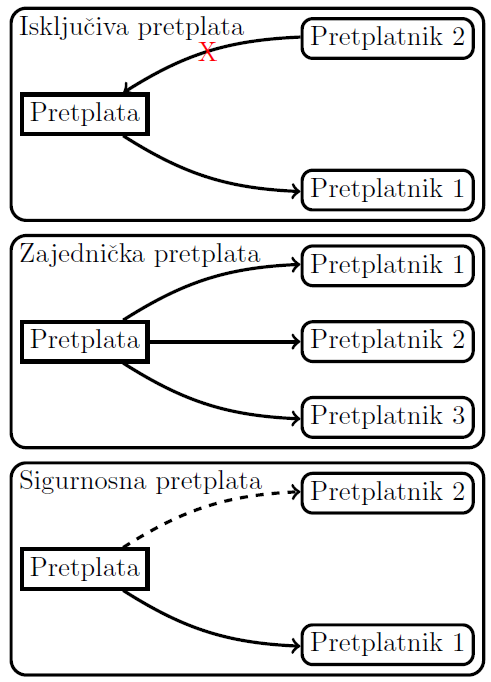
\includegraphics[max width=0.8\textwidth, max height=0.6\textwidth]{PulsarSubscription.png}
    \caption{Pulsar pretplate}
    \label{fig:pulsar-subscription}
\end{figure}

Kako objavljivači usmjeravaju dostavu poruka na pretince tako pretplatnici čitaju poruke koristeći pretplate \engl{subscription}. Slika \ref{fig:pulsar-subscription} prikazuje tri vrste pretplata. Isključiva pretplata \engl{exclusive subscription} pravo čitanja poruka daje samo jednom pretplatniku. Ako drugi pretplatnik pokuša čitati iz isključive pretplate on će biti odbijen. Zajednička pretplata \engl{shared subscription} jednoliko dostavlja poruke pretplatnicima. Svaka poruka dostavit će se samo jednom pretplatniku. Zajednička pretplata ne podržava skupnu potvrdu dostave poruka niti pazi na vremensko uređenje dostave poruka. Sigurnosna pretplata \engl{failover subscription} pravo čitanja daje samo jednom pretplatniku dok se pretplatniku ne dogodi ispad. Kada se dogodi ispad drugotni pretplatnik će nastaviti čitanje poruka od mjesta ispada.

\subsection{Posrednik}

Posrednik je program bez stanja koji se sastoji od dva dijela. Prvi dio je poslužitelj s REST sučeljem za upravljanje i pretraživanje tema, a drugi dio je otpravnik \engl{dispatcher} za prijenos podataka. Umjesto da objavljivači i pretplatnici izravno razgovaraju s posrednikom mogu se spojiti na zastupnika \engl{proxy} koji će preusmjeriti njihove zahtjeve posrednicima. Posrednik može odbaciti udvostručene poruke tako da ih ne proslijedi zapisničarima.

Pulsar grozdovi mogu umnožiti poruke ako pripadaju istom procesu. Zadaća posrednik je poslužiti poruke pretplatnicima iz upravljane knjige ili BookKeeper zapisničara, dok je ZooKeeper nadzornik zadužen za čuvanje podata o grozdu. Zapisničar zapisuje poruke koje su poslane posredniku.

\subsection{Upravljana knjiga}

BookKeeper grozd je raspodijeljeni zapisivač koji se sastoji od barem jednog zapisničara \engl{bookie}. Zapisničar zapisuju poruke koje mu posrednici pošalju. Poruke se mogu umnožiti i zapisati u više knjiga odjednom. Svaka tema sastoji se od barem jedne knjige \engl{ledger}. Kapacitet poruka može se povećati dodavanjem zapisničara. Zapisničari mogu istovremeno čitati i pisati poruke.

Knjiga je struktura podatka u koju se poruke mogu dodati samo na kraj. Nakon što se knjiga zatvori ona se jedino može čitati. Ako se zapisničaru dogodi ispad, knjiga se zatvori. Kada se ispad otkloni zapisničar će ustanoviti u kojem je stanju knjiga i ustanovljeno stanje poslati ostalim zapisničarima u grozdu.

Upravljana knjiga \engl{managed ledger} je skup BookKeeper knjiga u koju se upisuju poruke koje pripadaju jednoj temi. Iako se poruke mogu zapisati u samo jednu knjigu više BookKeeper knjiga olakšava brisanje i pisanje poruka. Upravljana knjiga sastoji se od skupa tokova podataka koji se zapisuju u knjigu s jednim pisačem i skupa pokazivača koji prate koje poruke su pretplatnici pročitali. Zapisivač prije pisanja poruke u upravljanu knjigu poruke zapisuje u dnevnik.

\subsection{Pretplatnik}

Pretplatnik je korisnički program koji se pretplaćuje na pretplatu teme. Postoje tri vrste pretplate. Svaka pretplata određuje način na koji pretplatnik čita poruke. Pretplatnik može ili biti blokiran dok posrednik ne dobije poruku ili nastaviti s radom i dobiti budućnostnicu \engl{future} kojom će čitati poruke. Pretplatnik može pojedinačno ili skupno potvrditi poruke \engl{batch acknowledge}.

Ako korisnik nije zadovoljan izvedenim pretplatnikom on može koristiti sučelje čitača. Sučelje čitača je biblioteka koja omogućuje ručno potvrđivanje poruka, ponovno čitanje poruke i odbacivanje umnoženih poruka.


\section{Usporedba}

\begin{table}[H]

\begin{adjustwidth}{-15mm}{15mm}

\begin{tabular}{|l|l|l|}
\hline
                            & \textbf{Kafka}                & \textbf{Pulsar}                                \\ \hline
Programski jezik            & Scala/Java                    & Java                                           \\ \hline
Nadziranje grozda           & ZooKeeper                     & ZooKeeper                                      \\ \hline
Zapisivanje podataka        & Kafka                         & BookKeeper                                     \\ \hline
Umotvorine                  & tema, pretinac                & tema, pretinac, segment                        \\ \hline
Teme                        & memorijske                    & memorijske, nepostojane                        \\ \hline
Identifikator poruke        & odmak                         & logički                                        \\ \hline
Odmak                       & cijeli broj                   & Pulsar pokazivač                               \\ \hline
Zapis odmaka                & Kafka tema                    & zapisničar                                     \\ \hline
Pretplate                   & skup pretplatnika             & isključiva, zajednička, sigurnosna             \\ \hline
Potvrđivanje poruka         & skupno                        & pojedinačno ili skupno                         \\ \hline
Garancija objave            & barem jednom                  & "kao jednom"                                   \\ \hline
Garancija pretplate         & barem jednom                  & "kao jednom"                                   \\ \hline
Umnožavanje poruka          & vođa-sljedbenici              & zapisničari                                    \\ \hline
Jedinica paralelizma        & pretinac                      & pretplata                                      \\ \hline
Izolirano pisanje i čitanje & ne                            & da                                             \\ \hline
Ograničenje pretinca        & manje od broja posrednika     & nema                                           \\ \hline
Ograničenje pretplatnika    & manje od broja pretinaca      & nema                                           \\ \hline
Gubitak poruka              & ispad N od N posrednika       & ispad N od N zapisničara                       \\ \hline
Brisanje poruka             & istek vremena                 & složeno                                        \\ \hline
Geo-umnožavanje             & MirrorMaker                   & podržano                                       \\ \hline
Posredničko spajanje        & nema                          & podržano                                       \\ \hline
Sažimanje                   & podržano                      & podržano                                       \\ \hline
Razine administracije teme  & nema                          & stanar, područje imena                         \\ \hline
Usmjeravanje poruka         & ne                            & ne                                             \\ \hline
\end{tabular}

\end{adjustwidth}
 
\caption{Usporedba Apache Kafka i Apache Pulsar}
\label{table:kafka_pulsar}

\end{table}



\chapter{Specifikacija sakupljača vrijednosti}

Apache Kafka pokreće se u okruženju s drugim sustavima. Okruženje je opisano pretpostavkama koje su nepromjenjive i uvijek vrijede. Zahtjevi su svojstva i mogućnosti programa koje je poželjno ali nije potrebno ispuniti.


\section{Pretpostavke}

\begin{itemize}
    \item Nadzirani sustav i sakupljač vrijednosti koriste siguran intranet
    \item Postoji više od deset Kafka grozdova i više od sto Kafka posrednika
    \item Kafka posrednici raspodijeljeni su na velik broj računala
    \item Kafka grozdovi i posrednici mogu se pokrenuti i završiti s radom u bilo kojem trenutku
    \item Može se dogoditi ispad, ali ne i bizantski \citep{kafka-docs}
\end{itemize}


\section{Zahtjevi}

\begin{itemize}
    \item Sakupljač vrijednosti se jednostavno umnoži i nije pozadinski proces
    \item Sakupljač vrijednosti samostalno pronalazi nove Kafka grozdove i posrednike
    \item Sakupljač vrijednosti šalje nadzirane vrijednosti s malim zakašnjenjem od trenutka očitavanja
    \item Sakupljač vrijednosti očitava nadzirane vrijednosti svake sekunde ili češće
    \item Sakupljač vrijednosti zapisuje nadzirane vrijednosti u Kafka temu
    \item Sakupljač vrijednosti oslobađa računalne resurse kada se nadzirani sustav ugasi
    \item Nadzirane vrijednosti imaju jedinstvenu oznaku nadziranog sustava iz kojeg su pročitane
    \item Nadzirane vrijednosti imaju vremensku oznaku kada su pročitane
\end{itemize}



\chapter{Postojeći sakupljači vrijednosti}

Istraživanje postojećih rješenja ima višestruku ulogu: usporediti mane i prednosti izvedenog rješenja; naučiti zašto i kako su drugi riješili problem; ponovno iskoristiti ili unaprijediti postojeće rješenje za rješavanje novog problema. U nadi da postoji rješenje koje zadovoljava većinu ili sve zahtjeve sustava istraženi su mali programi i veliki sustavi.


\section{Jolokia}

\begin{figure}[H]
    \centering
    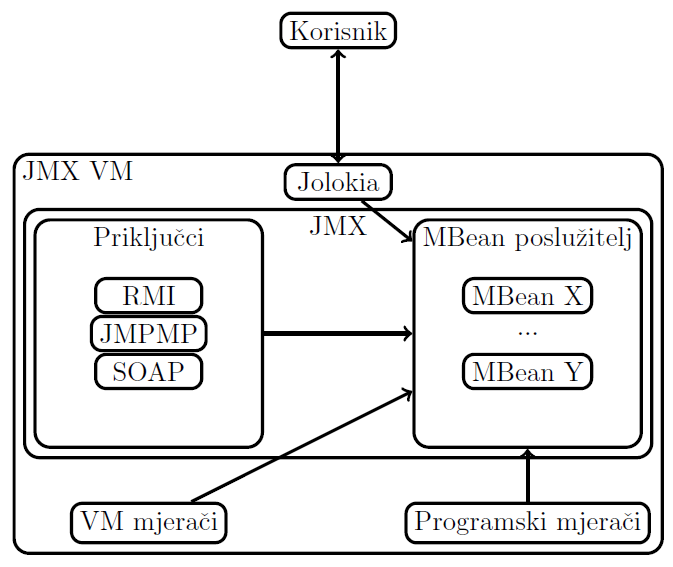
\includegraphics[max width=0.8\textwidth, max height=0.6\textwidth]{Jolokia.png}
    \caption{Arhitektura Jolokie}
    \label{fig:jolokia}
\end{figure}

Jolokia \citep{jolokia} je most između JMX i HTTP. Jolokia se pokreće kao agent u Java VM ili kao samostojeći poslužitelj. Slika \ref{fig:jolokia} prikazuje izvršavanje upita. HTTP upit postavi se Jolokiji koja skriva komplicirano dobavljanje nadziranih vrijednosti iza jednostavne funkcije. Nadzirane vrijednosti Jolokia šalje korisniku u JSON obliku.

Jolokia je vrlo jednostavno i učinkovito rješenje za nadziranje Java programa. Nažalost, Jolokia krši zahtjeve pozadinskog procesa i samostalnog pronalaženja novih Kafka grozdova i posrednika. Ako se Jolokia pokrene kao agent ona se pokrene kao poseban pozadinski proces na računalu na kojem se nalazi nadzirani sustav. Ako se pokrene kao samostojeći poslužitelj ona neće znati kada je novi Kafka grozd ili posrednik pokrenut jer nema načina da Jolokiji dojave pokretanje.


\section{Prometheus}

Prometheus \citep{prometheus} je potpuno rješenje za nadziranje proizvoljnih programa. Slika \ref{fig:prometheus} prikazuje dijelove Prometheusa: poslužitelj, vremenska baza podataka i sakupljač nadziranih vrijednosti. Sakupljač mjerače nalazi samostalno ili koristi otkrivatelja. Kada sakupljač pročita vrijednosti one se pohrane u bazu podataka i u stalnu memoriju. Prije prikazivanja ili stvaranja uzbune korisnici mogu izabrati podskup vrijednosti jezikom PromQL koji je nalik SQLu.

\begin{figure}[H]
    \centering
    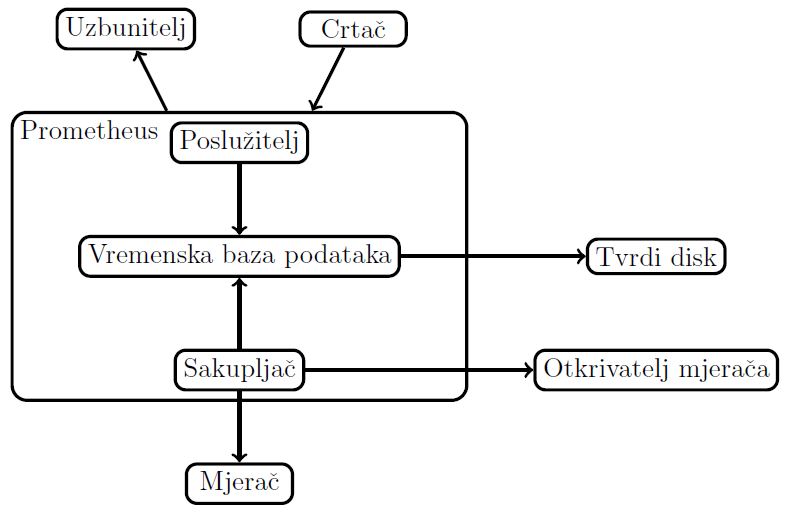
\includegraphics[max width=0.8\textwidth, max height=0.6\textwidth]{Prometheus.png}
    \caption{Arhitektura Prometheusa}
    \label{fig:prometheus}
\end{figure}

\newpage
Velika prednost i nedostatak Prometheusa je njegov opseg. Problem zahtjeva samo nadzor, a ne predočavanje, obradu i zapisivanje podataka. Prometheus također dugo čeka između očitanja nadziranih vrijednosti. Zahtjev traži čitanje svakih sekundu ili manje, a Prometheus čeka par sekundi.


\section{Confluent sakupljač vrijednosti}

Confluent sakupljač vrijednosti \citep{confluent-metrics-reporter} je dodatak na Kafka grozd i posrednika. Sakupljač čita i šalje nadzirane vrijednosti u Kafka temu nadziranog ili nekog drugog grozda. Svi novi Kafka posrednik pokreće se s Confluent sakupljačem.

Confluent sakupljač vrijednosti ispunjuje sve zahtjeve. Nije pozadinski proces jer dolazi u obliku JAR datoteke koja se pokreće i prestaje s radom Kafka grozda i posrednika te šalje nadzirane vrijednosti visokom frekvencijom. Nažalost, Confluent sakupljač vrijednosti je zatvoreno rješenje koje se ne može nadograditi, poboljšati ili proširiti.



\chapter{Arhitektura sakupljača vrijednosti}

Postoji velika rasprava kako oblikovati programski sustav \citep{clean-code} \citep{code-complete}. Sustav se oblikuje na razini okoline, rješenja, projekta, razreda, funkcije i naredbe. Okolina je skup pretpostavki o računalu, operacijskom sustavu, postojećim sustavima i mreži. Rješenje je skup projekata koji zajedno rješavaju problem. Projekt je program koji ispunjava podskup zahtjeva sustava. Razred je skup podatka i funkcija koje djeluju nad njima u objektno orijentiranoj paradigmi, a skup funkcija u proceduralnoj paradigmi.


\section{Okolina}

\begin{figure}[H]
    \centering
    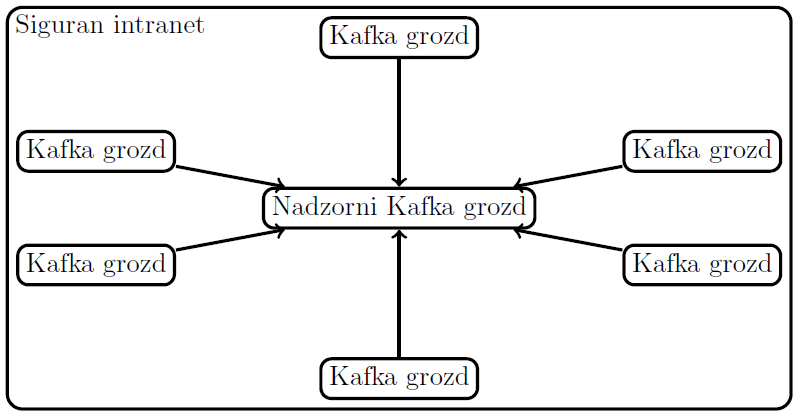
\includegraphics[max width=0.8\textwidth, max height=0.6\textwidth]{KafkaEnvironment.png}
    \caption{Okolina sustava}
    \label{fig:kafka-environment}
\end{figure}

Slika \ref{fig:kafka-environment} prikazuje mali podskup Kafka grozdova. Grozdovi koriste sigurni intranet za međusobni razgovor. Napadač ne postoji i ne može izazvati ispad pogrešnim korištenjem programa. Grozd može iskusiti ispad. Kafka grozdovi mogu se pokrenuti i završiti s radom u bilo kojem trenutku. Dijelovi grozda raspodijeljeni su na više računala. Kafka grozdovi šalju nadzirane vrijednosti u središnji nadzorni Kafka grozd. Nadzorni grozd je otporan na ispade i fizički odvojen od ostalih grozdova.


\section{Arhitektura rješenja}

Slika \ref{fig:collectors} prikazuje kako sakupljači vrijednosti nadziru Kafka posrednike. Kafka grozd sastoji se od barem jednog Kafka posrednika i ZooKeeper nadzornika. Posrednici šalju poruke pretplatnicima i zapisuju poruke objavljivača. Nadzornik zapisuje podatke o grozdu. Svaki posrednik ima svoj sakupljač vrijednosti. Kada se pokrene posrednik pokrene se i sakupljač vrijednosti. Sakupljač vrijednosti sastoji se od tri projekta: KaSta, Zook i JMXMan. KaSta pita Zook kojeg posrednika treba nadzirati. Zatim KaSta od JMXMan saznaje nadzirane vrijednosti. Svi KaStae šalju nadzirane vrijednosti u udaljeni nadzorni Kafka grozd.

\begin{figure}[H]
    \centering
    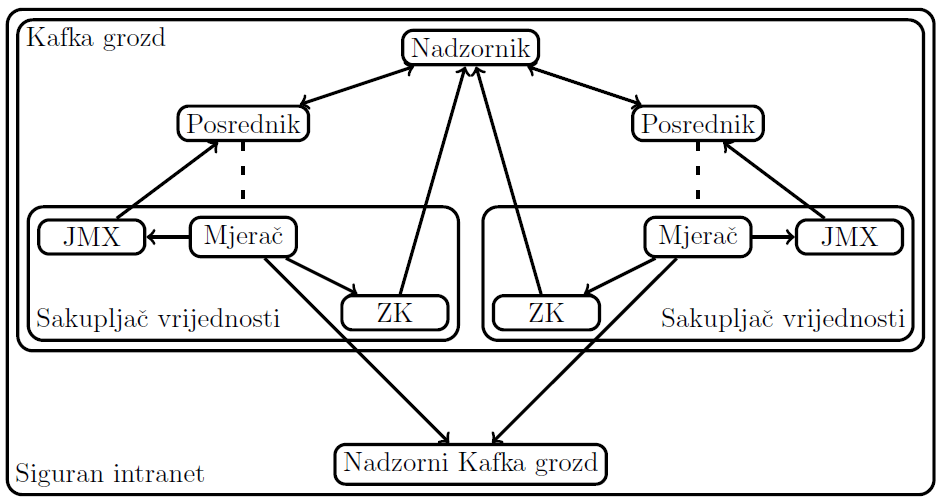
\includegraphics[max width=0.8\textwidth, max height=0.6\textwidth]{KafkaCollectors.png}
    \caption{Nadzor jednostavnog Kafka grozda}
    \label{fig:collectors}
\end{figure}


\section{Arhitektura projekt}

Rješenje je podijeljeno na projekte gdje svaki ispunjuje disjunktni podskup zahtjeva sustava. Projekti se mogu nadograditi i promijeniti bez utjecaja na druge projekte. U malom projektu od nekoliko razreda lakše je naći grešku nego u velikom projektu. Projekte je primjereno izvesti na objektno orijentirani način jer su njihove strukture podataka poznate, a funkcije nisu.

\subsection{Arhitektura Zook}

\begin{figure}[H]
    \centering
    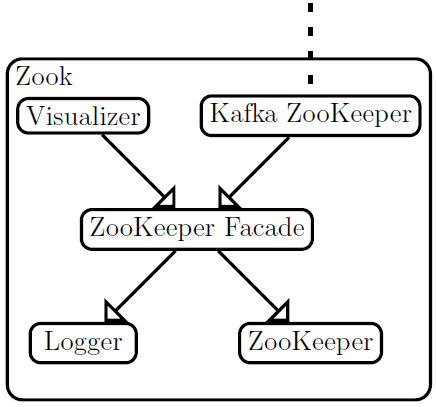
\includegraphics[max width=0.8\textwidth, max height=0.6\textwidth]{Zook.png}
    \caption{Odnosi Zook razreda}
    \label{fig:zookeeper-kafka}
\end{figure}

\begin{itemize}
    \item Visualizer - zadužen za predočavanje podataka u ZooKeeper čvorovima
    \item Kafka ZooKeeper - zadužen za pojednostavljenje odnosa između Kafka posrednika i ZooKeeper nadzornika
    \item ZooKeeper Facade - zadužen za pojednostavljenje razgovora s ZooKeeper nadzornikom
    \item Logger - zadužen za ispisivanje događaja
    \item ZooKeeper - zadužen za izvršavanje ZooKeeper naredbi
\end{itemize}

\subsection{Arhitektura JMXMan}

\begin{figure}[H]
    \centering
    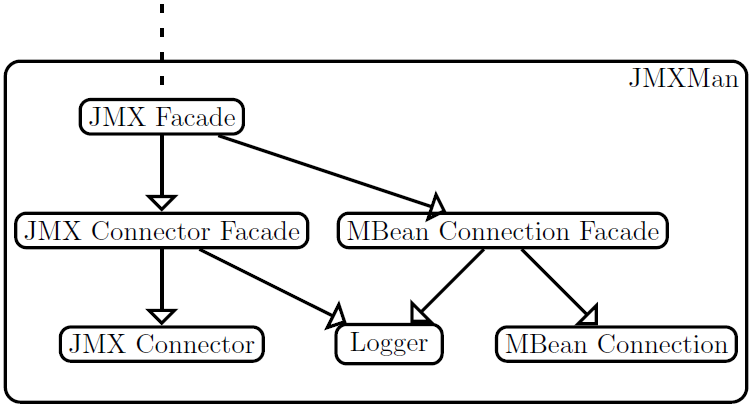
\includegraphics[max width=0.8\textwidth, max height=0.6\textwidth]{JMXMan.png}
    \caption{Odnosi JMXMan razreda}
    \label{fig:jmx-client}
\end{figure}

\begin{itemize}
    \item JMX Facade - zadužen za pojednostavljenje Java Management Extensions (JMX) sustava
    \item JMX Connector Facade - zadužen za pojednostavljenje JMX priključka
    \item MBean Connection Facade - zadužen za pojednostavljenje korištenja Managed Beans (MBean)
    \item JMX Connector - zadužen za izvršavanje JMX naredbi
    \item Logger - zadužen za ispisivanje događaja
    \item MBean Connection - zadužen za izvršavanje MBean naredbi
\end{itemize}

\subsection{Arhitektura KaSta}

\begin{figure}[H]
    \centering
    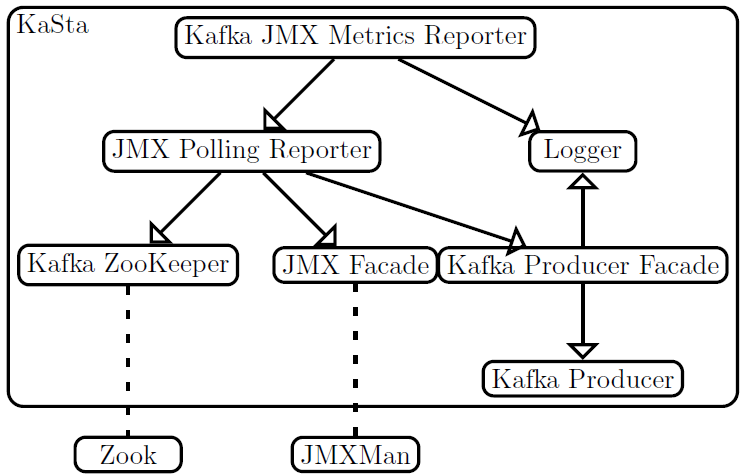
\includegraphics[max width=0.8\textwidth, max height=0.6\textwidth]{KaSta.png}
    \caption{Odnosi KaSta razreda}
    \label{fig:kafka-metrics-reporter}
\end{figure}

\begin{itemize}
    \item Kafka JMX Metrics Reporter - zadužen za pokretanje sakupljača vrijednosti
    \item JMX Polling Reporter - zadužen za očitavanje nadziranih vrijednosti
    \item Logger - zadužen za ispisivanje događaja
    \item Kafka ZooKeeper - zadužen za pojednostavljenje odnosa između Kafka posrednika i ZooKeeper nadzornika
    \item JMX Facade - zadužen za pojednostavljenje Java Management Extensions (JMX) sustava
    \item Kafka Producer Facade - zadužen za pojednostavljenje slanja poruka u Kafku
    \item Kafka Producer - zadužen za izvršavanje naredba objavljivača
\end{itemize}



\chapter{Izvedba sakupljača vrijednosti}

Rješenje je izvedeno u programskom jeziku Java uz pomoć razvojnog okruženje Eclipse. Apache Maven je sustav za upravljanje Java projektima: izgradnja, upravljanje ovisnosti i izrada dokumentacije. Apache Kafka je nadzirani sustav za kojeg je izgrađen sakupljač vrijednosti, dok je Apache ZooKeeper pomoćni sustav kojim se Kafka koristi za nadzor Kafka grozda.

\begin{itemize}
    \item Java, inačica 1.8, openjdk 10.0.2
    \item Eclipse IDE, inačica 2018-2019, 4.9.0
    \item Apache Maven, inačica 3.6
    \item Apache Kafka, inačica 2.1
    \item Apache ZooKeeper, inačica 3.14
\end{itemize}


\section{Izvedba rješenja}

Rješenje koristi Apache Maven dodatke. Izvršni projekt mjerača koristi Maven Shade Plugin za pakiranje rješenja u "debelu" JAR datoteku, rješenje koje sa sobom nosi strane biblioteke, ovisnosti. Dodatku se navodi koje inačice stranih biblioteka treba pakirati s rješenjem. Izabrane biblioteke i inačice su one koje koristi Kafka. Ako se koriste pogrešne biblioteke ili inačice sakupljač vrijednosti izazvat će grešku prilikom pokretanja Kafka. Svi projekti, ZK, JMX i mjerač, koriste "Maven Compiler Plugin" za ograničavanje Java inačice. Ako se Java inačica ne ograniči može nastati greška prilikom izgradnje ili pokretanja projekta.

Stil pisanja Java projekata prati Google Java Style Guide osim ako nije drugačije navedeno.

\newpage
Prije izvedbe konačnog rješenja sagrađen je prototip. Prototip je program koji se odbaci nakon što izvođača nauči koristiti prototipirani sustav.

Projekt trguje robusnost za ispravnost. Robusnost mjeri koliko program dobro radi nakon što nastane greška. Ispravnost je svojstvo programa da radi točno kako je navedeno u zahtjevima. Za sakupljača vrijednosti je važnije da radi točno nego da nastavi raditi ako iskusi grešku.

Rješenje će "glasno" prijaviti grešku da korisniku privuče pažnju. 

Zbog načina izvedbe, Kafka će pokrenuti sakupljača vrijednosti prije nego završi pokretanje same sebe. Zato sakupljač vrijednosti čeka zadano vrijeme prije početka sakupljanja vrijednosti.


\section{Izvedba projekata}

\begin{lstlisting}[floatplacement=H]
:kasta
\--- :broker
|    \--- :JMXPollingReporter
|    \--- :KafkaJMXMetricsReporter
|    \--- :KafkaJMXMetricsReporterMBean
\--- :error
|    \--- :NeutralValues
|    \--- :Validator
\--- :external
|    \--- :ConfigNames
|    \--- :ConfigParser
|    \--- :DefaultValues
\--- :json
|    \--- :JacksonFacade
\--- :logging
|    \--- :LoggingFacade
\--- :producer
     \--- :KafkaProducerFacade
     \--- :KafkaProducerFacadeConfig
     \--- :Metric
     \--- :ProducerRecordFacade
\end{lstlisting}

\begin{itemize}
    \item Razred KafkaJMXMetricsReporter pokreće Apache Kafka. Kafka se pokreće u procesu iz kojeg se stvara dretva za razred. Dretva razreda otpustit će se kada Kafka procesa završi s radom.
    \item Uslijed greške funkcija ne vraća NULL vrijednost već neutralnu vrijednost pretpostavljenu u razredu NeutralValues. Vraćanje neutralne vrijednosti je preciznije od vraćanja NULL vrijednosti.
    \item Vrijednosti postavka su pretpostavljene u razredu DefaultValues. Pretpostavljene vrijednosti olakšavaju korištenje projekta.
    \item Projekti ne koristi skraćenice osim ako nisu opće poznate i rasprostranjene poput: IP, JMX ili MBean.
\end{itemize}


\section{Izvedba razreda}

\begin{lstlisting}[floatplacement=H, language=Java, caption={Projekt JMXMan}, captionpos=b, basicstyle=\footnotesize, numbers=left, stepnumber=1, backgroundcolor=\color{backcolour}, keywordstyle=\color{blue}, breaklines]
/**
 * Responsible for simplifying JMX interactions.
 */
public class JMXFacade implements AutoCloseable, IMBeanConnectionFacade {
 private JMXConnectorFacade connector;
 private MBeanConnectionFacade mbean_connection;

 public JMXFacade(JMXConnectorFacadeConfig config) {...}
 private JMXConnectorFacade createConnector(JMXConnectorFacadeConfig config) {...}
 private MBeanConnectionFacade createMBeanConnection() {...}
  
 public List<JMXMetric> getMetrics(Set<ObjectName> mbean_names) {...}
  
 public Set<ObjectName> getAllMBeanNames() {...}
 public List<String> getMBeanAttributeNames(ObjectName mbean_name) {...}
 public Map<String,String> getMBeanAttributeValueMap(ObjectName mbean_name, List<String> attributes) {...}
 
 @Override
 public void close() {...}
}
\end{lstlisting}

\begin{itemize}
    \item Razredi su imenice gdje svaka ima samo jednu disjunktnu dužnost. Redci 1-4 opisuju dužnost razreda.
    \item Redci 5-6 prikazuju kako razred koristi kompoziciju umjesto nasljeđivanja. Duge lance naslijeđenih razreda teško je promijeniti jer su razredi strogo ovisni. Prednost kompozicije nad nasljeđivanjem je lakoća promjene.
    \item Razredi pozivaju samo vlastite funkcije u redcima 9, 10, 12 i funkcije objekata koje su stvorile u redcima 14, 15, 16. Na ovaj način razredi znaju vrlo male o izvedbi drugih razreda.
    \item Razredi koji koriste računalne resurse oslobađaju iste neposredno nakon zadnjeg poziva funkcije u retku 19.
    \item Razredi pročelja pojednostavljuju korištenje stranih biblioteka. Strane biblioteke imaju razrede od kojih rješenje koristi samo mali podskup svih funkcija. Fasade omotaju funkcije zbog lakoće korištenja, izmjena i izolacije od promjena strane biblioteke.
    \item Razredi izbjegavaju vremensku ovisnost. Vremenska ovisnost nastaje kada razred očekuje da će korisnik pozvati funkcije određenim redoslijedom. Ovisnost se izbjegne izvedbom razreda s malim brojem funkcija koje je moguće pozvati bilo kojim redoslijedom.
    \item Redoslijed funkcija u razredu određen je njihovom apstraktnošću. Najapstraktniji korisnički razred koji poziva više izvršnih funkcija je na vrhu razreda. Ispod njega slijede, u redoslijedu pozivanja, ostale korisničke i izvršne funkcije.
\end{itemize}


\section{Izvedba funkcija}

\begin{lstlisting}[floatplacement=H, language=Java, caption={Razred JMX Connector Facade}, captionpos=b, basicstyle=\footnotesize, numbers=left, stepnumber=1, backgroundcolor=\color{backcolour}, keywordstyle=\color{blue}]
private void connect() {
 boolean is_not_connected = true;
 while (is_not_connected) {
  try {
   this.connector.connect(this.config.jmx_config);
   is_not_connected = false;
  } catch (IOException e) {
   e.printStackTrace();
      
   this.sleepBeforeConnecting();
  }
 }
}
\end{lstlisting}

\begin{itemize}
    \item Funkcija je omotač funkcije iz strane biblioteke u retku 5. Ako se funkcija omota, koristi na mnogo mjesta i strana biblioteka se promijeni, tada se promjena treba izvršiti samo u funkciji omotaču.
    \item Ako funkcija prima više od dva parametra, parametri se omotaju u strukturu podataka i pozivaju kao u retku 5. Ovako je funkcija kraća i čitljivija.
\end{itemize}

\begin{lstlisting}[floatplacement=H, language=Java, caption={Predikatna funkcija}, captionpos=b, basicstyle=\footnotesize, numbers=left, stepnumber=1, backgroundcolor=\color{backcolour}, keywordstyle=\color{blue}]
public static boolean isBrokerJmxPortOpen(String jmx_port) {
 boolean is_open = true;
 if (jmx_port.equals(BadValues.JMX_PORT)) {
  is_open = false;
 }
 return is_open;
}
\end{lstlisting}

\begin{itemize}
    \item Ime predikatnih, Booleovih funkcija i varijabli imaju prefiks "is" kao u retku 1.
    \item Redak 6 je jedina naredba za kraj izvođenja. Lakše je analizirati funkciju ako postoji samo jedna točka gdje funkcija završava.
    \item Funkcija radi samo jednu stvar. Naziv funkcije definira što je "jedna stvar". Korisničke funkcije koje pozivaju više izvršnih funkcija rade jednu stvar na visokoj razini apstrakcije, dok izvršne funkcije rade jednu stvar na razini izvedbe.
    \item Funkcije trebaju biti kratke, ne više od pet redaka. Kratke funkcije je lakše pročitati, izmijeniti i ponovno iskoristiti.
    \item Većina funkcija prima jedan ili nijedan parametar. Ako funkcija prima dva parametra, redoslijed parametara mora biti jasan iz naziva funkcije. Samodokumentirajuće funkcije je lakše koristiti bez čitanja dokumentacije.
\end{itemize}


\newpage
\section{Izvedba naredba}

\begin{lstlisting}[floatplacement=H, language=Java, caption={Razred Kafka ZooKeeper}, captionpos=b, basicstyle=\footnotesize, numbers=left, stepnumber=1, backgroundcolor=\color{backcolour}, keywordstyle=\color{blue}]
public List<String> getNodeChildren(String node_path) {
 List<String> node_children = NeutralValues.LIST;
 
 boolean is_watched = false;
 try {
  node_children = this.zookeeper.getChildren(node_path,is_watched);
 } catch (KeeperException | InterruptedException e) {
  e.printStackTrace();
 }

 return node_children;
}
\end{lstlisting}

\begin{itemize}
    \item Redci 1-12 sastoje se od jedne naredbe. Ako je više naredbi u jednom retku, onda su naredbe jednostavne: promjena primitivnog tipa podataka ili čitanje konstante. Kada se traže greške ili poboljšava funkcija, izmjenu je lakše napraviti ako su naredbe kratke i odvojene.
    \item Imena varijabli u redcima 1-12 dolaze iz domene problema, ne rješenja. Kada korisnici žele izmijeniti ili opisati problem, oni koriste riječi iz domene problema, dok programer koristi riječi iz domene rješenja. Zbog ovakvog imenovanja jaz između korisnika i programera je manji.
    \item U retku 2 koristi se konstanta. Konstante su imenovane i izdvojene u posebne razrede. Teško je odrediti sva mjesta na kojima se koristi ista konstanta ako ona nije izdvojena. Još teže je odrediti kako je izabrana vrijednost konstante.
    \item U retku 4 varijabla je definirana što kasnije kako bi opseg varijable bio što manji. Mali opseg povećava čitkost funkcije.
\end{itemize}



\chapter{Zaključak}

Raspodijeljeni sustavi su nepouzdani i zahtijevaju nadzor. Prvi korak u izgradnji programskog nadzora je sakupljač vrijednosti. Apache Kafka je popularni sustav za raspodijeljenu obradu tokova podataka nad kojim je izgrađen sakupljač vrijednosti. Prije izvedbe uspoređeni su postojeći alati za nadzora i sakupljanje vrijednosti. Postojeća rješenja su ili općenita i vrlo složena ili loše prilagođena za Kafka okolinu u kojoj se nadzirani posrednici često pokreću i završavaju s radom.

Sakupljač vrijednosti izveden je kao dodatak na Apache Kafka posrednika. Svaki posrednik ima svog sakupljača vrijednosti. Kada posrednik počne s radom i sakupljač počne s radom. Kada posrednik završi s radom i sakupljač završi s radom. Sakupljač se izvrsno skalira jer povećanje broja nadziranih posrednika ne utječe na brzinu rada programa. Sakupljač je sastavljen od tri projekta: Zook koji upravlja Apache ZooKeeperom, JMXMan koji izvršava JMX naredbe i KaSta koji čita i šalje nadzirane vrijednosti u udaljeni sustav na obradu. Pri izvedbi rješenja promjenjivost i jednostavnost su bile glavne ideje vodilje.

Sakupljač je jednostavno nadograditi i izmijeniti. U budućnosti moguće je nadograditi sakupljač tako da filtrira i pamti nadzirane vrijednosti. Trenutno se nadzirane vrijednosti šalju u udaljeni Kafka grozd ali moguće je razviti rješenje tako da podržava druge sustave. Projekti Zook i JMXMan mogu se također nadograditi bez utjecaja na sakupljač vrijednosti.



\chapter{Dodaci}


\section{Priručnik za korištenje sakupljača vrijednosti}

Sakupljač vrijednosti je složeno rješenje izgrađeno od nekoliko projekata. Kako bi korištenje sakupljača bilo lakše napisan je korisnički priručnik na engleskom jeziku. Priručnik je oblikovan koristeći Markdown reprezentacijski jezik kako bi se povećala čitljivost.

\begin{lstlisting}[breaklines]
## KaSta and KaMan User Guide

The guide will lead you through all the necessary steps in order to configure and run KaStaPull, KaSta and KaMan projects.  

This guide assumes KaSta and KaMan projects will be run on the CentOS 7 operating system.



### Preparing Kafka environment

You need to configure the environment at the hardware, operating system and application level.  

#### [Hardware](https://kafka.apache.org/documentation/#hwandos)

Your machine needs to have sufficient memory to run Kafka.  
I advise at least 4GB of RAM.  

#### [OS](https://kafka.apache.org/documentation/#os)

Kafka should work well on any Unix system and is tested on both Linux and Solaris.  
Avoid running Kafka on Windows.  

#### [Java version](https://kafka.apache.org/documentation/#java)

Kafka requires Java Development Kit (JDK) 1.8 or better to run.  
```
$: sudo yum install java
```



### Installing Kafka

After preparing the environment you are ready to install Kafka.  
I strongly advised you install Kafka in the [/opt directory](https://www.tldp.org/LDP/Linux-Filesystem-Hierarchy/html/opt.html).  

Download Kafka:  
```
$: sudo curl "https://www.apache.org/dist/kafka/2.1.1/kafka_2.11-2.1.1.tgz" -o /opt/kafka.tgz
```

Install Kafka:  
```
$: cd /opt/kafka
$: sudo mkdir kafka
$: sudo tar -xvzf /opt/kafka.tgz --strip 1
```

Uncomment a property in Kafka's server.properties:  
```
listeners=PLAINTEXT://:9092
```



### Running Kafka

Start ZooKeeper:  
```
$: sudo bin/zookeeper-server-start.sh config/zookeeper.properties
```

Start Kafka and open the JMX port:  
```
$: sudo JMX_PORT=Any-Free-Port bin/kafka-server-start.sh config/server.properties
```
There are many other methods of opening Kafka's JMX port. You can use whatever method you like.  

How do you know if you have opened Kafka's JMX port? Check ZooKeeper znode /brokers/ids.  



### Preparing KaSta and KaMan environment

#### [Git](https://git-scm.com/)

Install Git:  
```
sudo yum install git
```

#### [Maven](http://maven.apache.org/)

Install Maven:  
```
sudo yum install maven
```



### Preparing KaSta environment

#### Support projects

Download JMXMan:
```
$: cd /opt/projects
$: sudo git clone JMXMan-Project-URL jmxman
```

Download Zook:
```
$: cd /opt/projects
$: sudo git clone Zook-Project-URL zook
```

Install both projects with Maven:
```
$: cd /opt/projects/jmxman
$: sudo mvn install

$: cd /opt/projects/zook
$: sudo mvn install
```



### Installing KaSta

Download KaStaPull:  
```
$: cd /opt/projects
$: sudo git clone KaStaPull-Project-URL kastapull
```

Download KaSta:  
```
$: cd /opt/projects
$: sudo git clone KaSta-Project-URL kasta
```

Package KaStaPull into a JAR:  
```
$: cd /opt/projects/kastapull
$: sudo mvn package
```

Package KaSta into a JAR:  
```
$: cd /opt/projects/kasta
$: sudo mvn package
```



### Installing KaMan

Download KaMan:  
```
$: cd /opt/projects
$: sudo git clone KaMan-Project-URL kaman
```



### Architectural notes

Upon packaging KaStaPull, Maven will create a "fat" JAR with only JMXMan and Zook as dependencies. This behaviour is configured in Maven's pom.xml. Not doing so will crash Kafka due to a dependency conflict in Kafka's /libs.  

Example [pom.xml](https://gitlab.com/dataflux_group/backend/kasta-push/blob/master/pom.xml):
```
<build>
  <plugins>
    ...
    <plugin>
      <groupId>org.apache.maven.plugins</groupId>
      <artifactId>maven-shade-plugin</artifactId>
      <version>3.2.1</version>
      <configuration>
        <artifactSet>
          <includes>
            <include>aisoft:zook</include>
            <include>aisoft:jmxman</include>
          </includes>
        </artifactSet>
      </configuration>
      <executions>
        <execution>
          <phase>package</phase>
          <goals>
            <goal>shade</goal>
          </goals>
        </execution>
      </executions>
    </plugin>
    ...
  </plugins>
</build>
```



### Configuring KaStaPull

KaSta Connect JAR must be placed into /opt/connectors folder.
```
$: sudo cp /opt/projects/kastapull/target/kafkapull.jar /opt/connectors/
```

Optionally, you may also review the Connector properties in /opt/projects/kafkapull/target.



### Configuring KaSta

KaSta JAR must be placed into Kafka's /libs folder.
```
$: sudo cp /opt/projects/kasta/target/kasta.jar /opt/kafka/libs/
```

Append to Kafka's server.properties:
```
kafka.metrics.reporters=aisoft.kasta.broker.KafkaJMXMetricsReporter
```

Optionally, these properties may be appended as well:
```
reporter.delay.milliseconds=5000
reporter.interval.milliseconds=1000
metrics.kafka=localhost:9092
kafka.metrics.topic=jmx-metrics
```



### Configuring KaMan

Optionally, you may change properties in /opt/projects/kaman/target:
```
# Kafka AdminClient configuration
kaman.admin-timeout=2000
# Kafka future configuration
kaman.future-timeout=5000
```



### Running KaStaPull

After starting Kafka run:  
```
$: sudo /opt/kafka/bin/connect-standalone.sh /opt/kafka/config/connect-standalone.properties /opt/projects/kastapull/target/connector-config.properties
```



### Running KaSta

KaSta is ran when you run a Kafka broker. That's it!  



### Running KaMan

Run KaMan by executing:  
```
$: pwd
  /opt/projects/kaman
$: sudo mvn exec:java
```

Visit {machine_ip_host}:8080/swagger-ui.html or {machine_ip_host}:8080/kafka/{broker_ip_port} to start using KaMan.



### Supplementary guides

* [Official Kafka Quickstart](https://kafka.apache.org/quickstart)

* [DigitalOcean: Install Kafka on CentOS 7](https://www.digitalocean.com/community/tutorials/how-to-install-apache-kafka-on-centos-7)

\end{lstlisting}


\section{Kafka stablo podataka u ZooKeeperu}

ZooKeeper nadzornik zapisuje podatke u datotečni sustav koji nalikuje stablu. U nastavku je ispis stabla koje Kafka često koristi za sinkronizaciju grozda.

\begin{lstlisting}
:cluster
\--- :id
:controller_echo
:controller
:brokers
\--- :ids
|    \--- :0
|    \--- :1
|    \--- :2
\--- :topics
|    \--- :topic1
|    |    \--- :partitions
|    |         \--- :0
|    |              \--- :state
|    |         \--- :1
|    |              \--- :state
|    \--- :topic2
|         \--- :partitions
|              \--- :0
|                   \--- :state
\--- :seqid
:zookeeper
\--- :quota
:admin
\--- :delete_topics
:isr_change_notification
:consumers
:log_dir_event_notification
:latest_producer_id_block
:config
\--- :changes
\--- :clients
\--- :brokers
\--- :topics
|    \--- :topic1
|    \--- :topic2
\--- :users
\end{lstlisting}


\section{Kafka nadzirane vrijednosti}

Sakupljač vrijednosti čita i šalje Java Management Extensions vrijednosti u nadzorni Kafka grozd. Primjeri nadziranih vrijednosti ispisani su u nastavku.

\begin{lstlisting}[breaklines]
{"identifier":"localhost:2181/0",
"name":"kafka.network:type=RequestMetrics,name=ThrottleTimeMs,request=Produce",
"values":{"Mean":"0.04786324786324787",
          "StdDev":"1.7931803358139955",
          "75thPercentile":"0.0",
          "98thPercentile":"0.0",
          "Min":"0.0",
          "95thPercentile":"0.0",
          "99thPercentile":"0.0",
          "Max":"75.0",
          "999thPercentile":"0.0",
          "Count":"1755",
          "50thPercentile":"0.0"
         }
}

...

{"identifier":"localhost:2181/0",
"name":"kafka.network:type=RequestMetrics,name=ErrorsPerSec,request=LeaderAndIsr,error=NONE",
"values":{"RateUnit":"SECONDS",
          "OneMinuteRate":"0.8441818857364531",
          "EventType":"requests",
          "Count":"51",
          "FifteenMinuteRate":"0.2363690035582246",
          "FiveMinuteRate":"0.3134491059201686",
          "MeanRate":"0.5163893250564741"
         }
}
\end{lstlisting}



\bibliography{literatura}
\bibliographystyle{fer}



\begin{sazetak}

U radu razvijen je sakupljač vrijednosti za Apache Kafka, popularni sustav za raspodijeljenu obradu tokova podataka. Postojeći sakupljači vrijednosti nisu primjereni za raspodijeljeni nadzor. Novi sakupljač vrijednosti izgrađen je od tri projekta: Zook koji upravlja Apache ZooKeeperom, JMXMan koji izvršava JMX naredbe i KaSta koji čita i šalje nadzirane vrijednosti u udaljeni sustav na obradu. Sakupljač se izvrsno skalira jer povećanje broja nadziranih Kafka posrednika ne utječe na brzinu rada programa. Rješenje je lako nadograditi jer je jednostavno i modularno.

\kljucnerijeci{raspodijeljeni sustav, nadzor, Apache Kafka, nadzirana vrijednost}
\end{sazetak}



\engtitle{Real-Time Health Monitoring in Distributed Data Stream Processing System}
\begin{abstract}

This thesis developed a metrics reporter for Apache Kafka, a popular distributed streaming system. Existing monitoring solutions are not well suited for distributed monitoring. A new metrics reporter was constructed from three projects: Zook which manages Apache ZooKeeper, JMXMan which executes JMX queries and KaSta which polls and sends metrics to a remote monitoring system. The reporter scales very well because the increase in the number of Kafka brokers has no impact on the reporter's performance. The reporter can be easily extended because of its simplicity and modularity.

\keywords{distributed system, monitoring, Apache Kafka, metric}
\end{abstract}

\end{document}
